\documentclass{beamer}
\mode<presentation>
{
  \usetheme{Madrid}      % or try Darmstadt, Madrid, Warsaw, ...
  \usecolortheme{beaver} % or try albatross, beaver, crane, ...
  \usefonttheme{serif}  % or try serif, structurebold, ...
  \setbeamertemplate{navigation symbols}{}
  \setbeamertemplate{caption}[numbered]
} 
\usepackage{bm} %to add math symbol@?}
\usepackage{graphicx} %to include graphics%
\usepackage{longtable}
\usepackage{lscape}
\usepackage{float}
\usepackage{epsfig} % to include EPS figure
\usepackage{epstopdf} % to include EPS figure
\usepackage{ragged2e}
\usepackage{tabularx,booktabs} %to make table
\usepackage{ragged2e}
\usepackage{tikz}
\usetikzlibrary{arrows,positioning}
\usepackage{amsmath} %this is for equation
\usepackage{breqn} %this also for equation
\usepackage[english]{babel}
\usepackage[utf8x]{inputenc}
\usepackage{xcolor}
\usepackage{listings}
\lstset
{
    language=[LaTeX]TeX,
    breaklines=true,
    basicstyle=\tt\scriptsize,
    %commentstyle=\color{green}
    keywordstyle=\color{blue},
    %stringstyle=\color{black}
    identifierstyle=\color{magenta},
}

\title[RCT Finding]{Speaking Truth to Twitter}
\author{Team 3}
\institute{Hertie School of Governance}
\date{May 12, 2016}

\AtBeginSection[]
{
  \begin{frame}<beamer>
    \frametitle{Outline}
    \tableofcontents[currentsection,currentsubsection]
  \end{frame}
}

\begin{document}

\begin{frame}
  \titlepage
\end{frame}

\begin{frame}{Outline}
  \tableofcontents
\end{frame}


%----------Beginning of Slides----------%

\section{Implementing the RCT}
\begin{frame} {Main changes}
	\begin{itemize}
	\item focus exclusively on Trump (not Clinton and Trump) 
	\item Sample:treatment group:1000, control group: 4420 
	\item 10 individuals asked to be withdrawn during treatment. Effect measured thus ITT effect
	\end{itemize}
\end{frame}

\begin{frame}{Implementation}
	\begin{itemize}
	\item creation of 5 Twitter accounts with same 		profile picture and information but different names (\textbf{A, B, C, D, E}) 
	\item regular creation of Twitter Apps which were used to automatically tweet the treamtment groups
	\item tweets were sent time frame
	\end{itemize}
\end{frame}

\begin{frame}{Implementation}
		\begin{figure}
			\begin{centering}
  	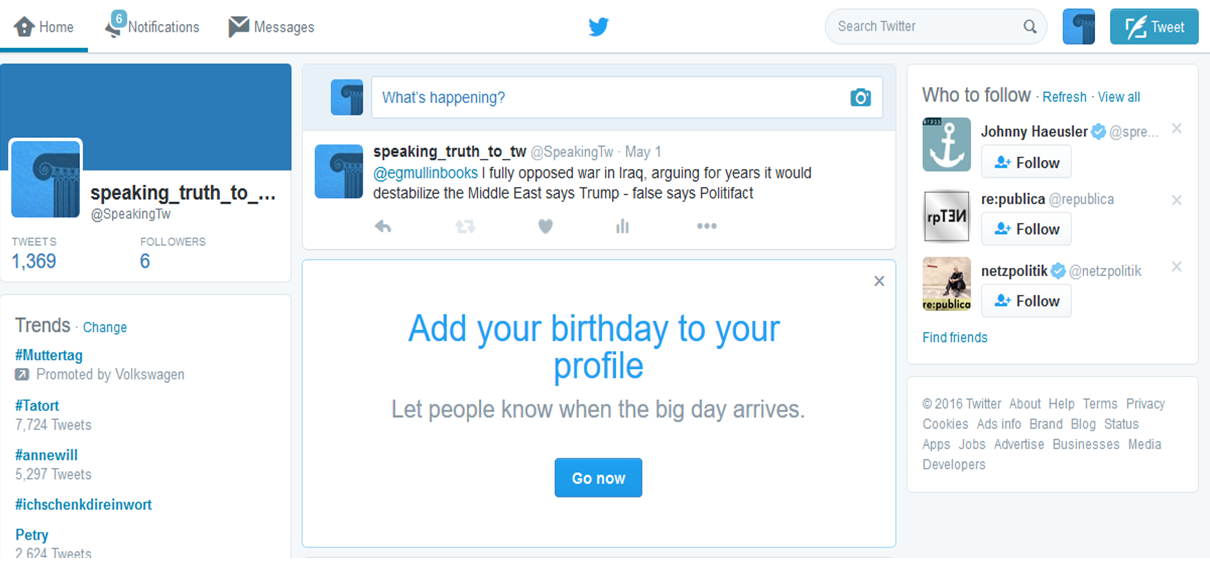
\includegraphics[scale=.45]{twitter_page.PNG}
  \caption{Twitter profile}
			\end{centering}
		\end{figure}
\end{frame}



\section{Some Descriptives}
\begin{frame}{Descriptives}
\begin{table}
		\begin{center}
	\tiny
	\begin{table}[ht]
\centering
\begin{tabular}{cp{6cm}cc}
  \hline
Tweet number & Text & Truth & Start date \\ 
  \hline
  1 & @LostinMemphis Trump says most wire transfers to Mexico from undocumented immigrants- half true says award-winning website Politifact &   0 & 2016-04-14 \\ 
    2 & @LostinMemphis Trump says his deficit to Clinton much smaller than Reagan's against Carter- false says award-winning website Politifact &  -2 & 2016-04-20 \\ 
    3 & @LostinMemphis Trump says Ted Cruz is mathematically out of winning the race - mostly true says politifact &   1 & 2016-04-22 \\ 
    4 & @LostinMemphis Trump says PA lost 35\%, and Harrisburg 40\%, of manufacturing jobs since 2001 - Mostly true says politifact &   1 & 2016-04-25 \\ 
    5 & @LostinMemphis Trump says football coach Rex Ryan won championships in NY twice - false says Politifact. He never did &  -2 & 2016-04-27 \\ 
    6 & @LostinMemphis Trump says ISIS makes millions of dollars a week by selling Libyan oil - false says Politifact &  -2 & 2016-04-29 \\ 
    7 & @LostinMemphis Trump says he fully opposed war in Iraq arguing for years it would destabilize the Middle East - false says Politifact &  -2 & 2016-04-30 \\ 
   \hline
\end{tabular}
\caption{Example tweets} 
\label{table:example_tweets}
\end{table}

	\end{center}
\end{table}	

%\item how many tweets (+ maybe list of the tweets)
%\item graph showing when the tweets were sent over the sample period 
%\item some information on the level of (unexpected) engagement of our treatment group with us (number of retweets and likes of our tweets, number of followers, number and examples of replies to our tweets)
\end{frame}

\begin{frame}{Descriptives}
	Information on our sample: table comparing the treatment and the control group containing for example the following things:


	\begin{itemize}
\item size of both groups (n)
\item twitter activity (likes\_n, tweets\_n) before the experiment
\item number of friends and/or followers
\item male/female (do we have that information?)
	\end{itemize}
\end{frame}
%-----------------------------------------------%



\section{Main Results: Data and Dependent Variables}
\begin{frame}{Results}
short detour on the data we collected throughout the entire time frame (specify time frame) → maybe we don’t actually need that on the slide, but just explain it. \textit{dependent variables (all per individual per day):}

\begin{itemize}
\item number of likes of tweets by Donald Trump
\item number of retweets of tweets by Donald Trump
\item number of tweets using the hashtag \textbf{\#MakeAmericaGreatAgain}
\item number of tweets including the key word \textsc{Trump} 
\end{itemize} 
\end{frame}


\section{Limitations}
\begin{frame}{Limitations}
\begin{itemize}

\item Self selection in the sample: 
\textit{Only active trump followers were selected in our study} and \textit{People had the option to opt-out}
\item Being recognized as a robot
\item Bias from manipulation of the twitter feed
\item Outcome is \textbf{likes} or \textbf{tweets} per day while the tweeting has been done at a certain time during the day...
\item Collinearity of variables in case of the lasting turn-on model!
\end{itemize}
\end{frame}




\begin{frame}{Interesting}
		\begin{figure}
			\begin{centering}
  	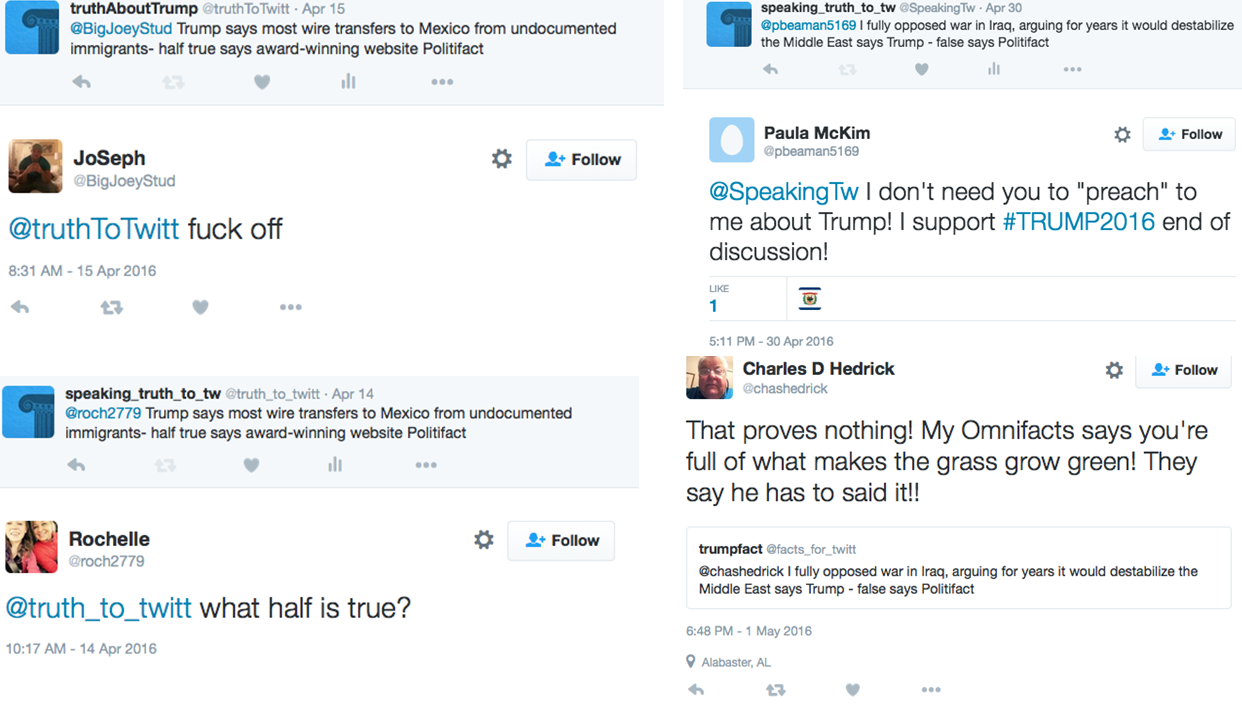
\includegraphics[scale=.45]{twitter_comment.PNG}
  \caption{Some interesting comments}
			\end{centering}
		\end{figure}
\end{frame}
		
\end{document}
